\chapter{BERTopic}
L'avvento dei moderni \emph{LLM} ha portato ad un'evoluzione del \textbf{NLP} (Natural Language Processing) con la conseguente nascita di nuovi framework e tecniche per le analisi più disparate.
Il \emph{topic modeling} non è esente da questo fenomeno, in particolare i modelli basati su \textbf{transformers} (cioè modelli che convertono testo in embeddings dipendenti dal contesto) si sono rilevati particolarmente efficaci.% nell'\emph{nlp}.
\textbf{Modelli preaddestrati} sono molto utilizzati perché permettono di creare rappresentazioni \textbf{accurate} e \textbf{rappresentative} di testi, potendo fare affidamento su dataset di training molto grandi e molto diversificati.
In questo contesto BERTopic è un \textit{framework} al passo con il corrente stato dell'arte, che offre alcuni vantaggi rispetto a tecniche antecedenti, fra cui permette di catturare il \textbf{significato semantico} dei documenti (riconosce ad esempio i sinonimi). Per dataset eterogenei e rumorosi come gli annunci di lavoro, questa capacità di individuare strutture semantiche latenti rende BERTopic una scelta particolarmente vantaggiosa rispetto ai modelli tradizionali. Inoltre in BERTopic specificare il il numero di classi è \textbf{opzionale}.
Inoltre BERTopic è composto da più \textit{submodules} con funzioni diverse, il che permette un'alta personalizzazione.

\section{Funzionalità}
All'interno di Bert Topic è possibile distinguere alcune funzionalità particolarmente utili per questo progetto:
\begin{enumerate}
\item Embedding
\item Dimensionality Reduction
\item Clustering
\item Tokenizer
\item c-TF-IDF
\end{enumerate}

BERTopic permette l'utilizzo di algoritmi diversi per ogni funzionalità, per personalizzare il proprio \emph{topic model}, ad esempio il clustering può essere effettuato da \emph{HDBSCAN} o da \emph{k-Means}.
Illustreremo ora tutti i moduli da noi usati, vedremo nello specifico la loro funzione e come la loro alterazione modifica il risultato finale.
\subsection{Embedding}
Il primo modulo è l'\textbf{embedder}, il cui compito è quello di trasformare i documenti in rappresentazioni numeriche.
i modelli principali consigliati nella documentazione\footnote{\url{https://maartengr.github.io/BERTopic/getting_started/embeddings/embeddings.html}} sono i \textbf{sentence transformers} (SBERT).
Ci sono molti modelli SBERT pre-addestrati tra cui scegliere, la documentazione ufficiale nei suoi esempi usa spesso all-MiniLM-L6-v2 un modello estremamente leggero e veloce, però non sufficientemente preciso nel catturare sfumature semantiche complesse o relazioni a lungo raggio.
paraphrase-MiniLM-L12-v2 e paraphrase-mpnet-base-v2, sono più accurati, ma più specializzati nel catturare relazioni di parafrasi, fra testi molto simili, sono inoltre inadatti a testi particolarmente lunghi come gli annunci di lavoro.
\textbf{all-mpnet-base-v2}, invece, ha una alta \textbf{precisione semantica}, e si comporta bene con documenti di lunghezza \textbf{medio-lunga}.
Ha però un limite di lunghezza di \textbf{512 token}. Con token in questo contesto ci riferiamo all' unità base che usano i modelli sentence transformers, composti da una parola o da una frazione di essa.
Ecco alcune informazioni sulla lunghezza del nostro dataset (dopo la pulizia):
\begin{figure}[H]
\centering
\scriptsize
\begin{tabular}{lccc}
\hline
 & n chars & n words & n tokens mpnet \\
\hline
count & 5357.00 & 5357.00 & 5357.00 \\
mean & 3315.48 & 457.92 & 594.54 \\
std & 1591.28 & 219.01 & 283.37 \\
min & 91.00 & 14.00 & 23.00 \\
50\% & 3087.00 & 427.00 & 554.00 \\
75\% & 4060.00 & 562.00 & 729.00 \\
90\% & 5213.40 & 717.00 & 934.00 \\
95\% & 6188.20 & 846.20 & 1103.40 \\
99\% & 8797.52 & 1203.44 & 1562.72 \\
max & 19470.00 & 2739.00 & 3753.00 \\
\hline
\multicolumn{4}{l}{Testi che superano i 512 token: 3075 (57.40\%)} \\
\multicolumn{4}{l}{Totale annunci: 5357} \\
\hline
\end{tabular}
\caption{Statistiche globali del dataset (totale annunci: 5357).}
\label{fig:dataset-stats}
\end{figure}
\noindent Quando SBERT riceve un input troppo lungo, lo \textbf{tronca} questo significa che applicando l'embedder così come è verrebbe tagliata una porzione molto grande del dataset.

\noindent Le prime opzioni che abbiamo considerato sono:
\begin{enumerate}
    \item Affidarsi ad un modello con un limite di dimensione input più alto (ad esempio \textbf{all-roberta-long-v1})
    \item Frammentare le descrizioni e fare il topic modeling in segmenti di quest'ultime.
\end{enumerate}
Il vantaggio della prima opzione è che i modelli \textit{long-context}, mantengono attenzione tra termini distanti, permettendo di cogliere relazioni semantiche a lungo raggio, cosa impossibile se si divide il testo in \textit{chunk}.
Non è però una caratteristica che abbiamo ritenuto significativa, data la natura del nostro \textit{dataset}, infatti i nostri paragrafi hanno natura scollegata, uno potrebbe parlare di competenze e un altro di mansioni, la coerenza globale è più importante in testi di natura \textbf{discorsiva}.
Inoltre se la lunghezza del testo è grande è probabile che contenga più temi, un unico embedding rischia di mescolare \textbf{sezioni semanticamente diverse}, ottenendo topic più grossolani.
La seconda opzione invece, oltre che generare topic più \textbf{puliti} e \textbf{interpretabili}, consente di aumentare molto il numero di documenti in input e questo è un vantaggio per dataset esegui come il nostro.
Però anche questo caso presenta delle criticità: non avremmo i topic relativi agli annunci come uniche entità, ma saranno relativi ai segmenti e andrebbero aggregati a posteriori per ottenere una \textbf{distribuzione di topic per annuncio}. In più in questo modo, gli annunci più lunghi avranno \textbf{più peso}, semplicemente perché hanno più paragrafi. La situazione si complica ulteriormente se i documenti contengono paragrafi simili, questo creerebbe dei \textbf{cluster} artefatti e quindi topic che non rispecchiano la natura del dataset. Un altro problema è che con questo metodo il modello è completamente ignaro della struttura globale dell'annuncio.
Questo approccio è più attuabile per risolvere un problema di \textbf{classificazione}, non per il \textit{topic modeling}.\medskip

\noindent La soluzione che abbiamo scelto è dunque quella di \textit{mean-max-pooling}.
\subsubsection{Mean-max pooling}

\noindent Con questa tecnica si ottiene un embedding per ogni annuncio partendo dagli embedding dei paragrafi, seguendo i passaggi seguenti:
\begin{enumerate}
    \item calcolare gli embedding di ciascun paragrafo;
    \item normalizzare ogni embedding;
    \item calcolare media aritmetica e massimo elemento per elemento;
    \item concatenare i due vettori risultanti;
    \item normalizzare nuovamente il vettore concatenato.
\end{enumerate}

In questo modo si ottiene un embedding unico di dimensione doppia rispetto l'output dell'embedder che può catturare sia il \textbf{significato generale} dell'annuncio, sia le \textbf{feature salienti} dei singoli paragrafi: queste due componenti possono produrre vettori più \textbf{discriminativi} e quindi più facilmente separabili nello spazio semantico.

Per attuare questo approccio serve inoltre una strategia di segmentazione degli annunci che soddisfi al contempo \textbf{coerenza semantica} e criteri di lunghezza: il segmento non può essere troppo corto, altrimenti SBERT non ha il contesto per estrarre topic singnificativi, e non può ovviamente superare la lunghezza massima consentita. Approfondiamo questo aspetto nel capitolo \textbf{Pre-processing}.
\subsection{Dimensionality Reduction}
I vettori generati dall'embedder hanno dimensione originale 768 e ciò potrebbe rendere difficile il \emph{clustering}. Per questo è importante introdurre nella pipeline un algoritmo di riduzione della dimensione.
L'idea di questi algoritmi è quella di ridurre la dimensione di un insieme di vettori preservandone la \textbf{struttura topologica locale}.
Di default BERTopic usa \textbf{UMAP}\footnote{\url{https://maartengr.github.io/BERTopic/getting_started/dim_reduction/dim_reduction.html}} per questo compito poiché \emph{preserva sia la struttura locale, che quella globale degli spazi ad alte dimensioni}.
UMAP lavora costruendo un \textit{grafo fuzzy locale}: ogni punto viene connesso ai suoi \texttt{n\_neighbors} più vicini e la connessione è pesata in base alla distanza. Questo grafo rappresenta la topologia locale dello spazio originale.
UMAP cerca poi una rappresentazione a bassa dimensione che minimizzi la differenza tra il grafo originale e il grafo proiettato.

L'obiettivo è mantenere la densità e la vicinanza dei punti simili, consentendo allo stesso tempo di contrarre regioni sparse.
Questo bilanciamento consente di preservare la struttura locale pur comprimendo lo spazio globale.
Vediamo più nel dettaglio questi punti.
\subsubsection{Fuzzy simplicial complex}
Per costruire il grafo iniziale ad alta dimensionalità, \textbf{UMAP} crea una struttura chiamata \textit{fuzzy simplicial complex}. In pratica, si tratta di una rappresentazione di un grafo pesato, in cui i pesi degli archi rappresentano la \textbf{probabilità che due punti siano connessi}.

Per determinare la connessione tra due punti, UMAP\footnote{\url{https://pair-code.github.io/understanding-umap/}} estende un \textbf{raggio locale} a partire da ciascun punto e collega i punti quando i rispettivi raggi si sovrappongono. La scelta di questo raggio è cruciale:
Se è troppo piccolo, il risultato sarà un insieme di \textbf{piccoli cluster isolati};
se è troppo grande, tutti i punti finiranno per essere \textbf{collegati tra loro}, perdendo così la struttura locale.

UMAP risolve questo problema scegliendo un raggio locale \textbf{adattivo}, basato sulla distanza rispetto al $k$-esimo vicino più prossimo di ciascun punto. Successivamente, il grafo viene reso ``sfumato'' (\textit{fuzzy}) diminuendo la probabilità di connessione man mano che la distanza aumenta.

Infine, imponendo che ogni punto sia connesso almeno al proprio vicino più prossimo, UMAP garantisce un equilibrio tra la \textbf{preservazione della struttura locale} e la \textbf{coerenza della struttura globale}.
\begin{figure}[H]
\centering
\includegraphics[width=0.75\textwidth]{img/BERTopic/umap/UMAP\_projection.png}
\caption{Proiezione UMAP nel piano bidimensionale. Dopo l'intersezione con il primo \emph{neighbour}, il cerchio diventa \emph{sfumato}, riducendo il peso della connessione.\protect\footnotemark}
\label{fig:umap-projection}
\end{figure}
\footnotetext{\url{https://pair-code.github.io/understanding-umap/}}
\subsubsection{Parametri}
I due parametri più importanti di UMAP sono \texttt{n\_neighbors} e \texttt{min\_dist}, poiché regolano l'equilibrio tra struttura \textit{locale} e \textit{globale} nella proiezione finale.\footnote{\url{https://pair-code.github.io/understanding-umap/}}

\paragraph{\texttt{n\_neighbors}.} Determina il numero di vicini utilizzato per costruire il grafo fuzzy iniziale. Valori bassi enfatizzano le relazioni locali, isolando micro-strutture anche molto sottili; valori alti favoriscono invece la coerenza complessiva, preservando maggiormente la geometria globale dell'insieme di punti.
Per visualizzare l'effetto di \texttt{n\_neighbors} consideriamo la proiezione bidimensionale di un modello 3D campionato con 50\,000 punti. Le immagini mostrano come la struttura globale emerga gradualmente all'aumentare del numero di vicini, mentre i dettagli fini sono preservati soltanto per valori più bassi.

\begin{figure}[H]
\centering
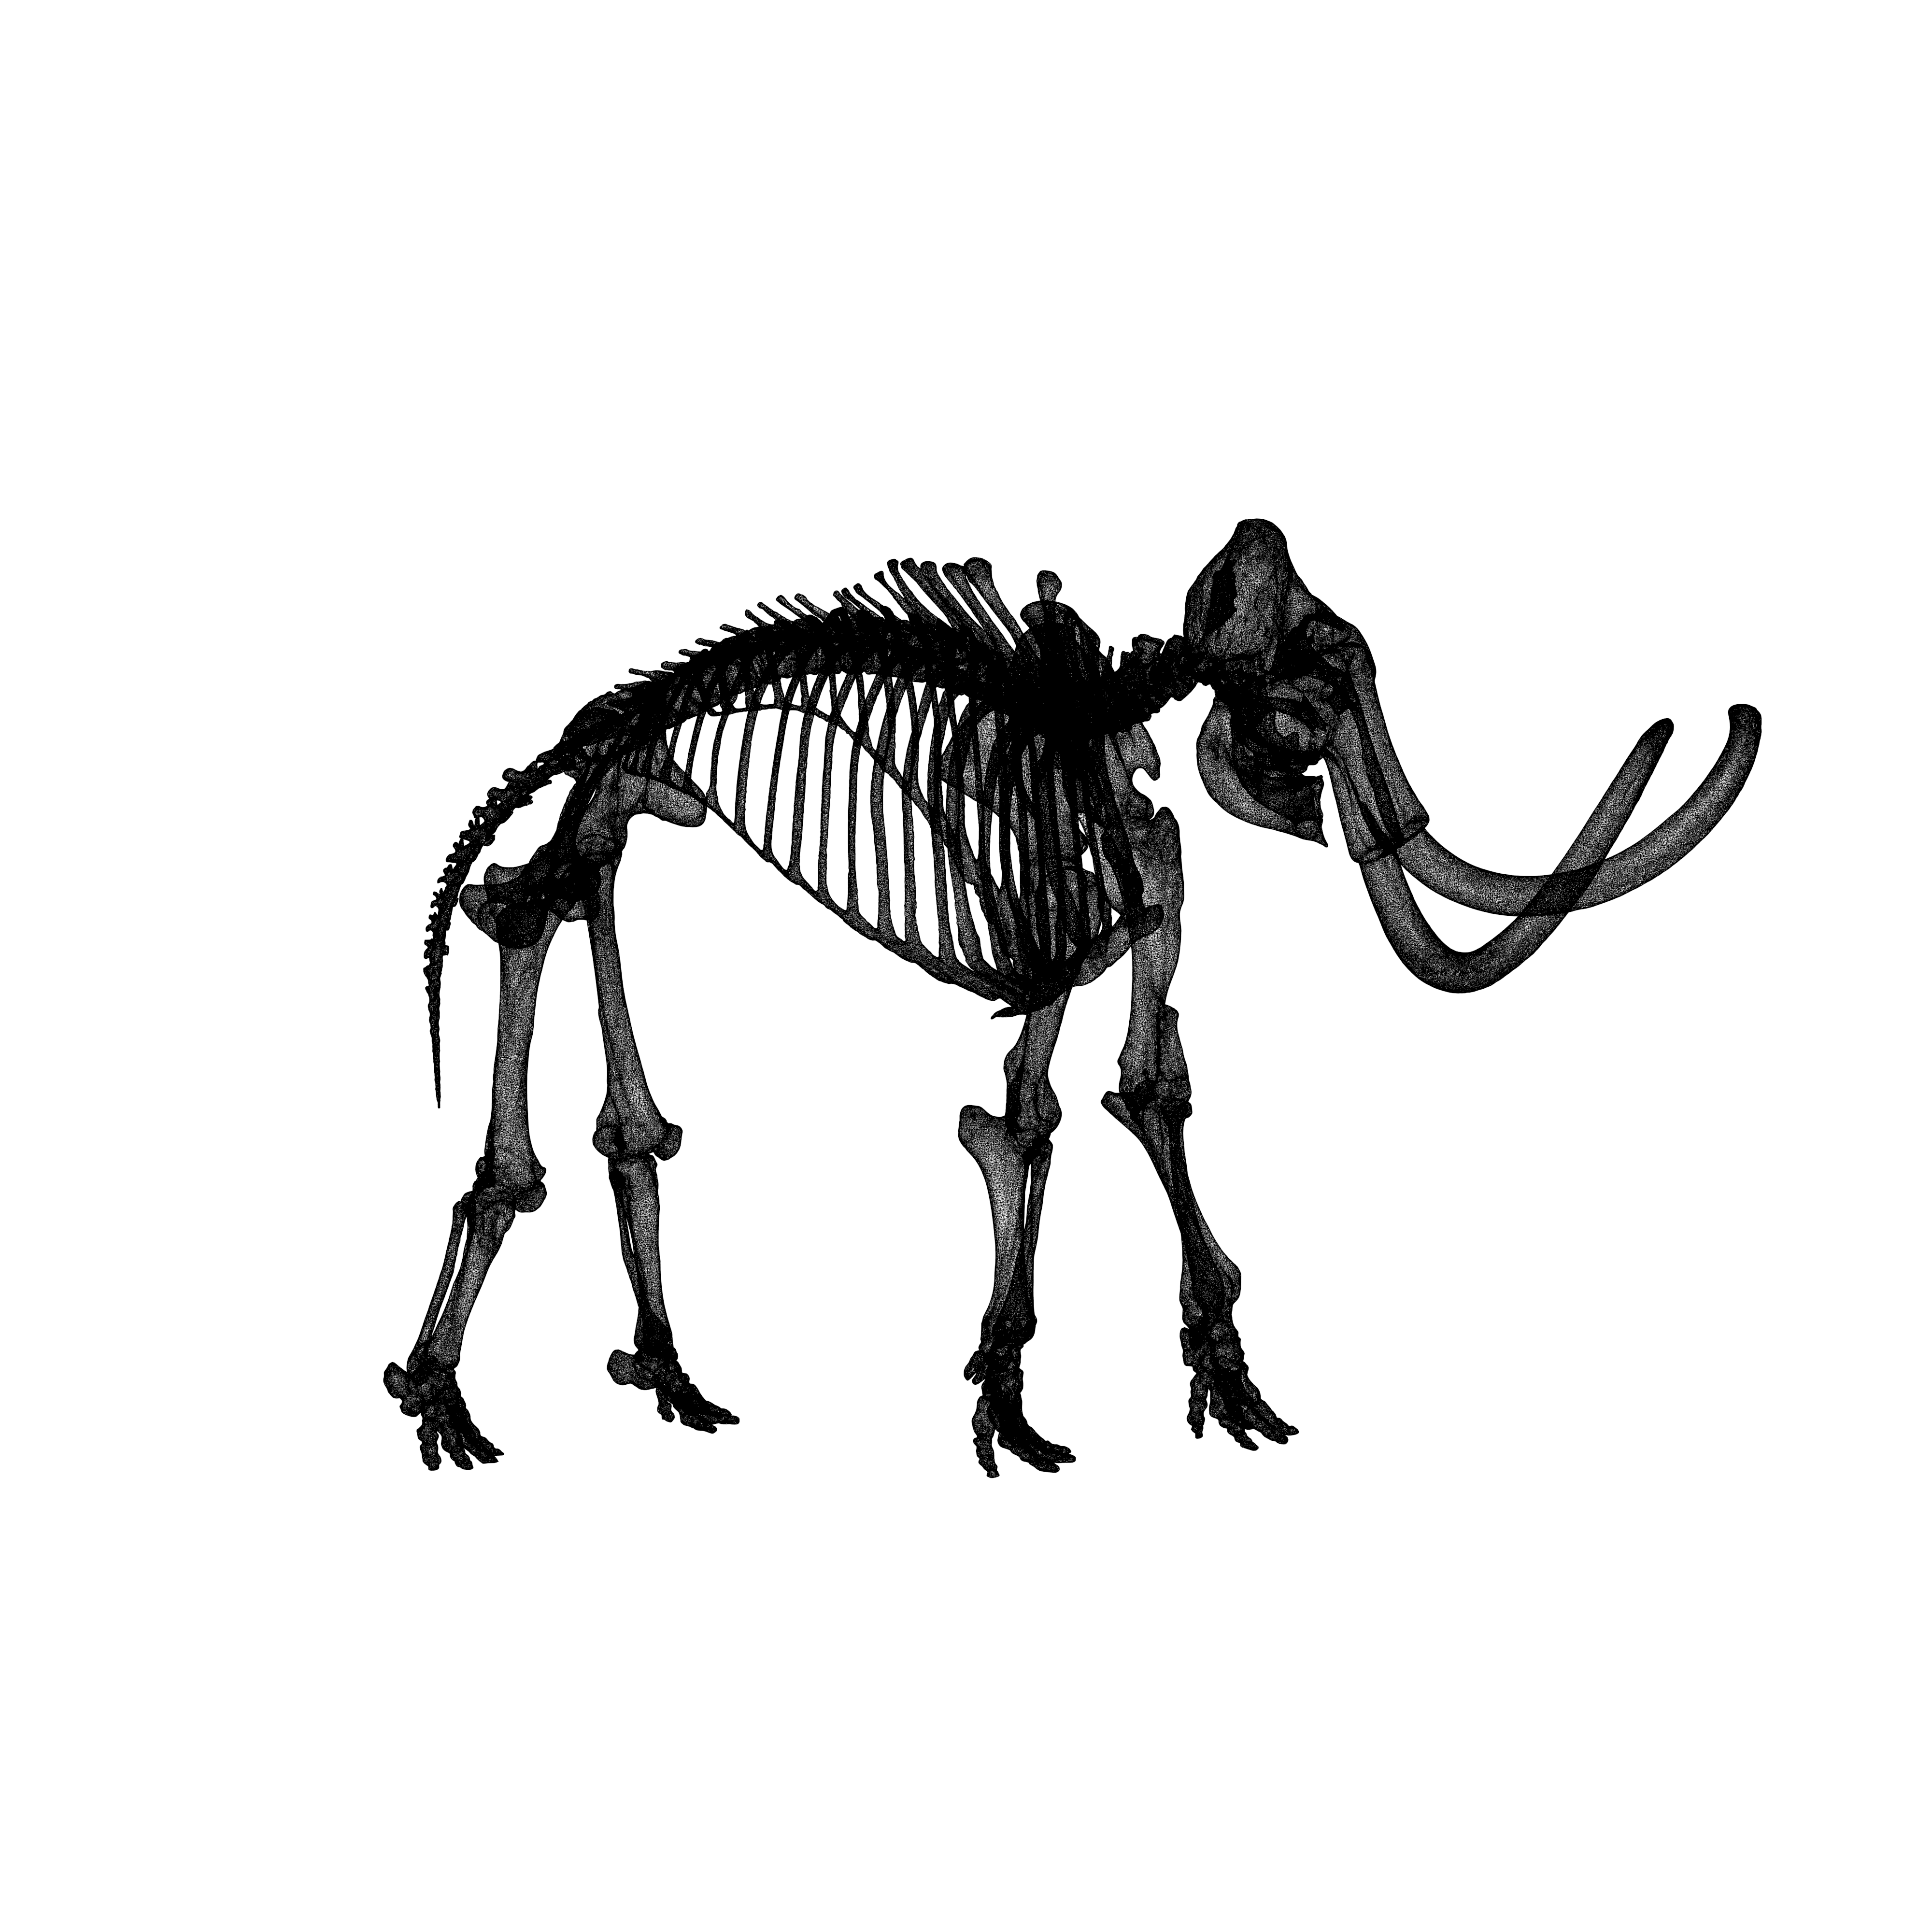
\includegraphics[width=0.5\textwidth]{BERTopic/umap/mammoth_render.png}

\begin{subfigure}{0.32\textwidth}
    \centering
    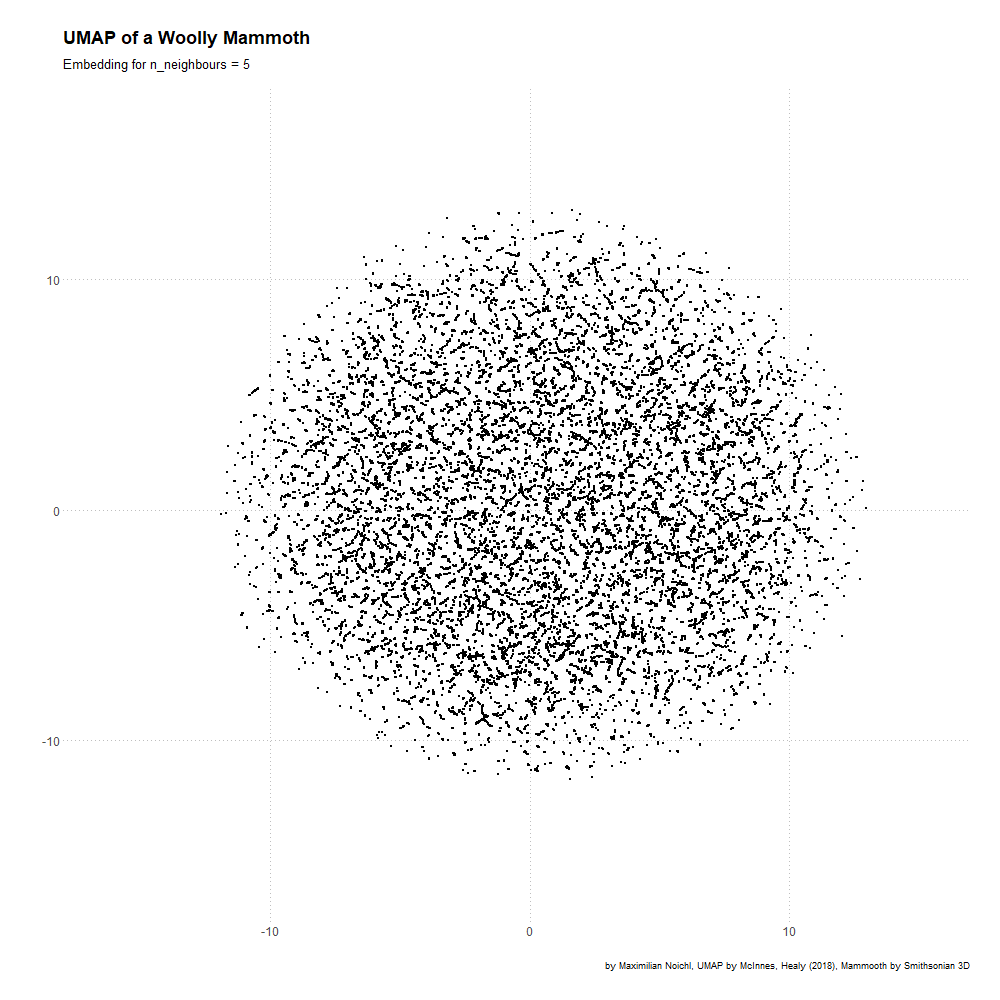
\includegraphics[width=\textwidth]{BERTopic/umap/n_neighbours5.png}
    \caption{$n\_neighbors = 5$}
\end{subfigure}\hfill
\begin{subfigure}{0.32\textwidth}
    \centering
    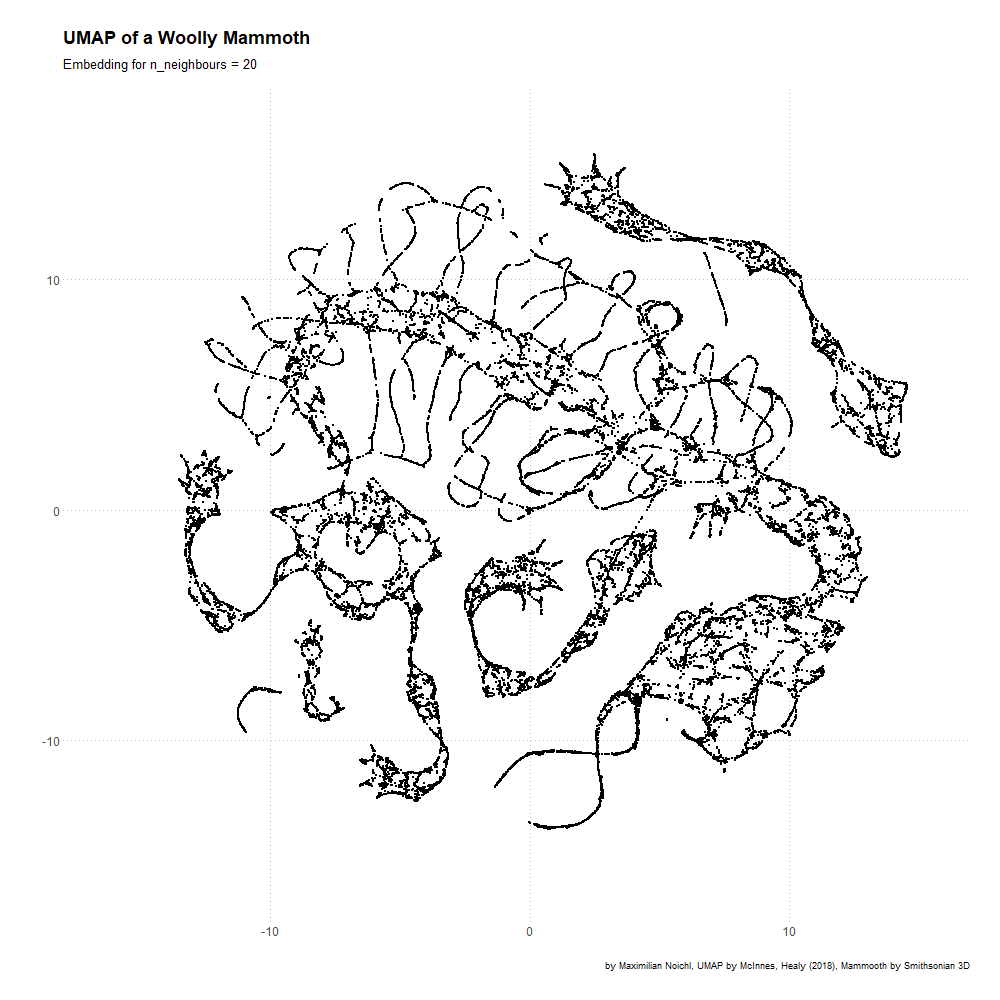
\includegraphics[width=\textwidth]{BERTopic/umap/n_neighbours20.png}
    \caption{$n\_neighbors = 20$}
\end{subfigure}\hfill
\begin{subfigure}{0.32\textwidth}
    \centering
    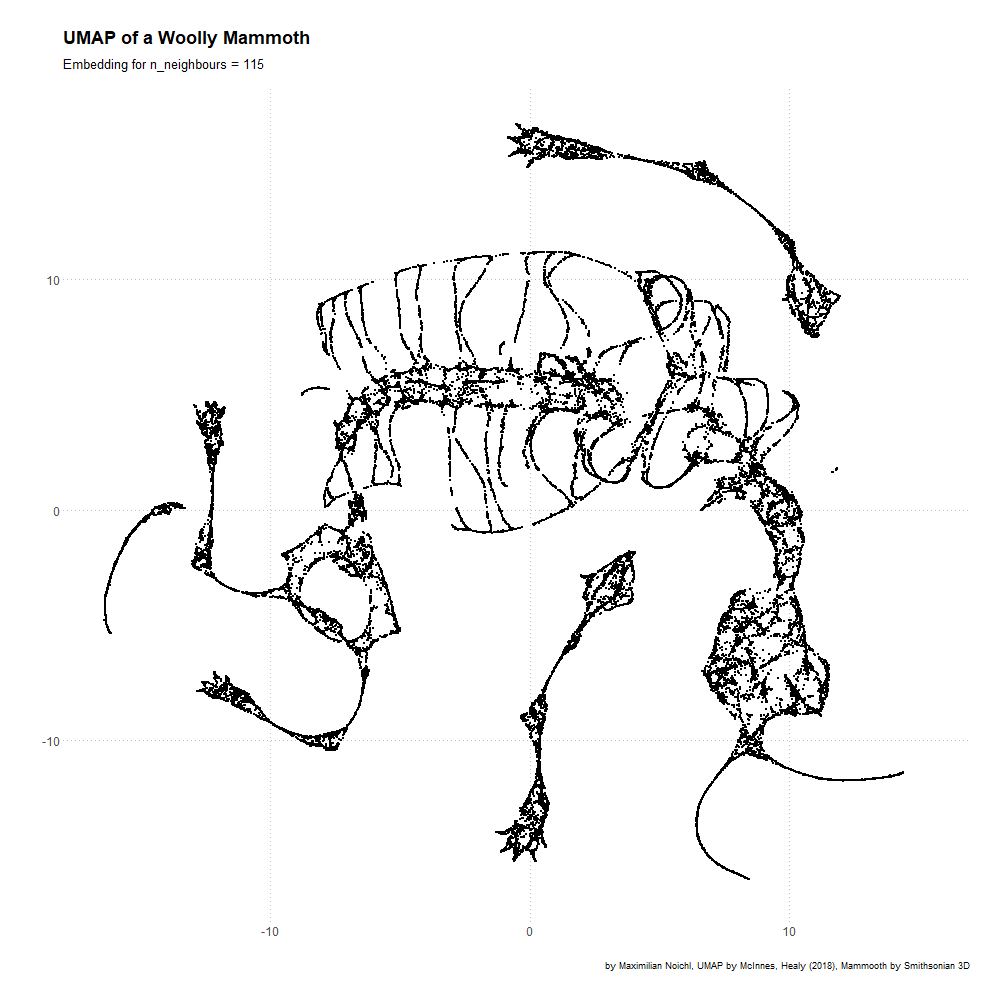
\includegraphics[width=\textwidth]{BERTopic/umap/n_neighbours115.png}
    \caption{$n\_neighbors = 115$}
\end{subfigure}
\caption{Proiezione UMAP di un modello 3D con 50\,000 punti in un piano 2D. Fonti: \href{https://3d.si.edu/object/3d/mammuthus-primigenius-blumbach:341c96cd-f967-4540-8ed1-d3fc56d31f12}{Smithsonian 3D Digitization Program} e \href{https://www.maxnoichl.eu/projects/mammoth/}{Max Noichl}.}
\label{fig:umap-mammoth}
\end{figure}
Si osservi come per valori ridotti di \texttt{n\_neighbors} la proiezione mantenga dettagli locali (curve delle zanne o delle zampe), ma perda la forma complessiva del mammut; all'aumentare del parametro la sagoma globale diventa riconoscibile, a scapito delle piccole variazioni geometriche. In modo analogo, sperimentare con valori come 15, 50 o 100 nel nostro dataset permette di calibrare il livello di granularità dei topic: valori molto bassi frammentano in gruppi minuti, mentre impostazioni alte tendono a fondere i cluster semantici più affini; una scelta intermedia (ad esempio \texttt{n\_neighbors} = 50) offre un equilibrio adeguato tra dettaglio locale e coerenza globale.
Per giungere a questa scelta sono stati provati diversi set di iperparametri; riportiamo di seguito quelli usati per la configurazione finale, così da facilitarne la riproducibilità:

\begin{lstlisting}[language=Python]
umap_model = UMAP(
    n_neighbors=n,
    n_components=10,
    min_dist=0.0,
    metric="cosine",
    random_state=1,
)
hdbscan_model = HDBSCAN(
    min_cluster_size=50,
    min_samples=15,
    metric="euclidean",
    cluster_selection_method="eom",
    prediction_data=True,
    cluster_selection_epsilon=0.1,
)
\end{lstlisting}

\begin{table}[H]
\centering
\footnotesize
\begin{tabular}{rrrrrr}
\hline
$n\_neighbors$ & $n\_topics$ & mean cluster size & std cluster size & topics $<100$ & topics $>500$ \\
\hline
15  & 15 & 208.87 & 267.01 & 8  & 2 \\
50  & 61 & 224.98 & 294.64 & 25 & 8 \\
60  & 62 & 197.81 & 254.00 & 26 & 6 \\
70  & 58 & 208.09 & 242.64 & 22 & 4 \\
100 & 2  & 2396.50 & 2090.91 & 0  & 2 \\
\hline
\end{tabular}
\caption{Sintesi degli esperimenti al variare di $n\_neighbors$: numero di topic trovati, dimensione media e deviazione standard dei cluster, oltre al conteggio dei topic piccoli ($<100$ documenti) e molto grandi ($>500$ documenti).}
\label{tab:n-neighbors-summary}
\end{table}

\noindent Nel corso dei test abbiamo variato \texttt{n\_neighbors} tra i valori 15, 50, 60 e 70 (con un confronto a 100 come baseline), scegliendo infine \texttt{n\_neighbors} = 50 come compromesso ottimale; la Tabella~\ref{tab:n-neighbors-summary} riassume il numero di topic e la distribuzione delle dimensioni dei cluster ottenuti in ciascun caso.

\begin{figure}[H]
\centering
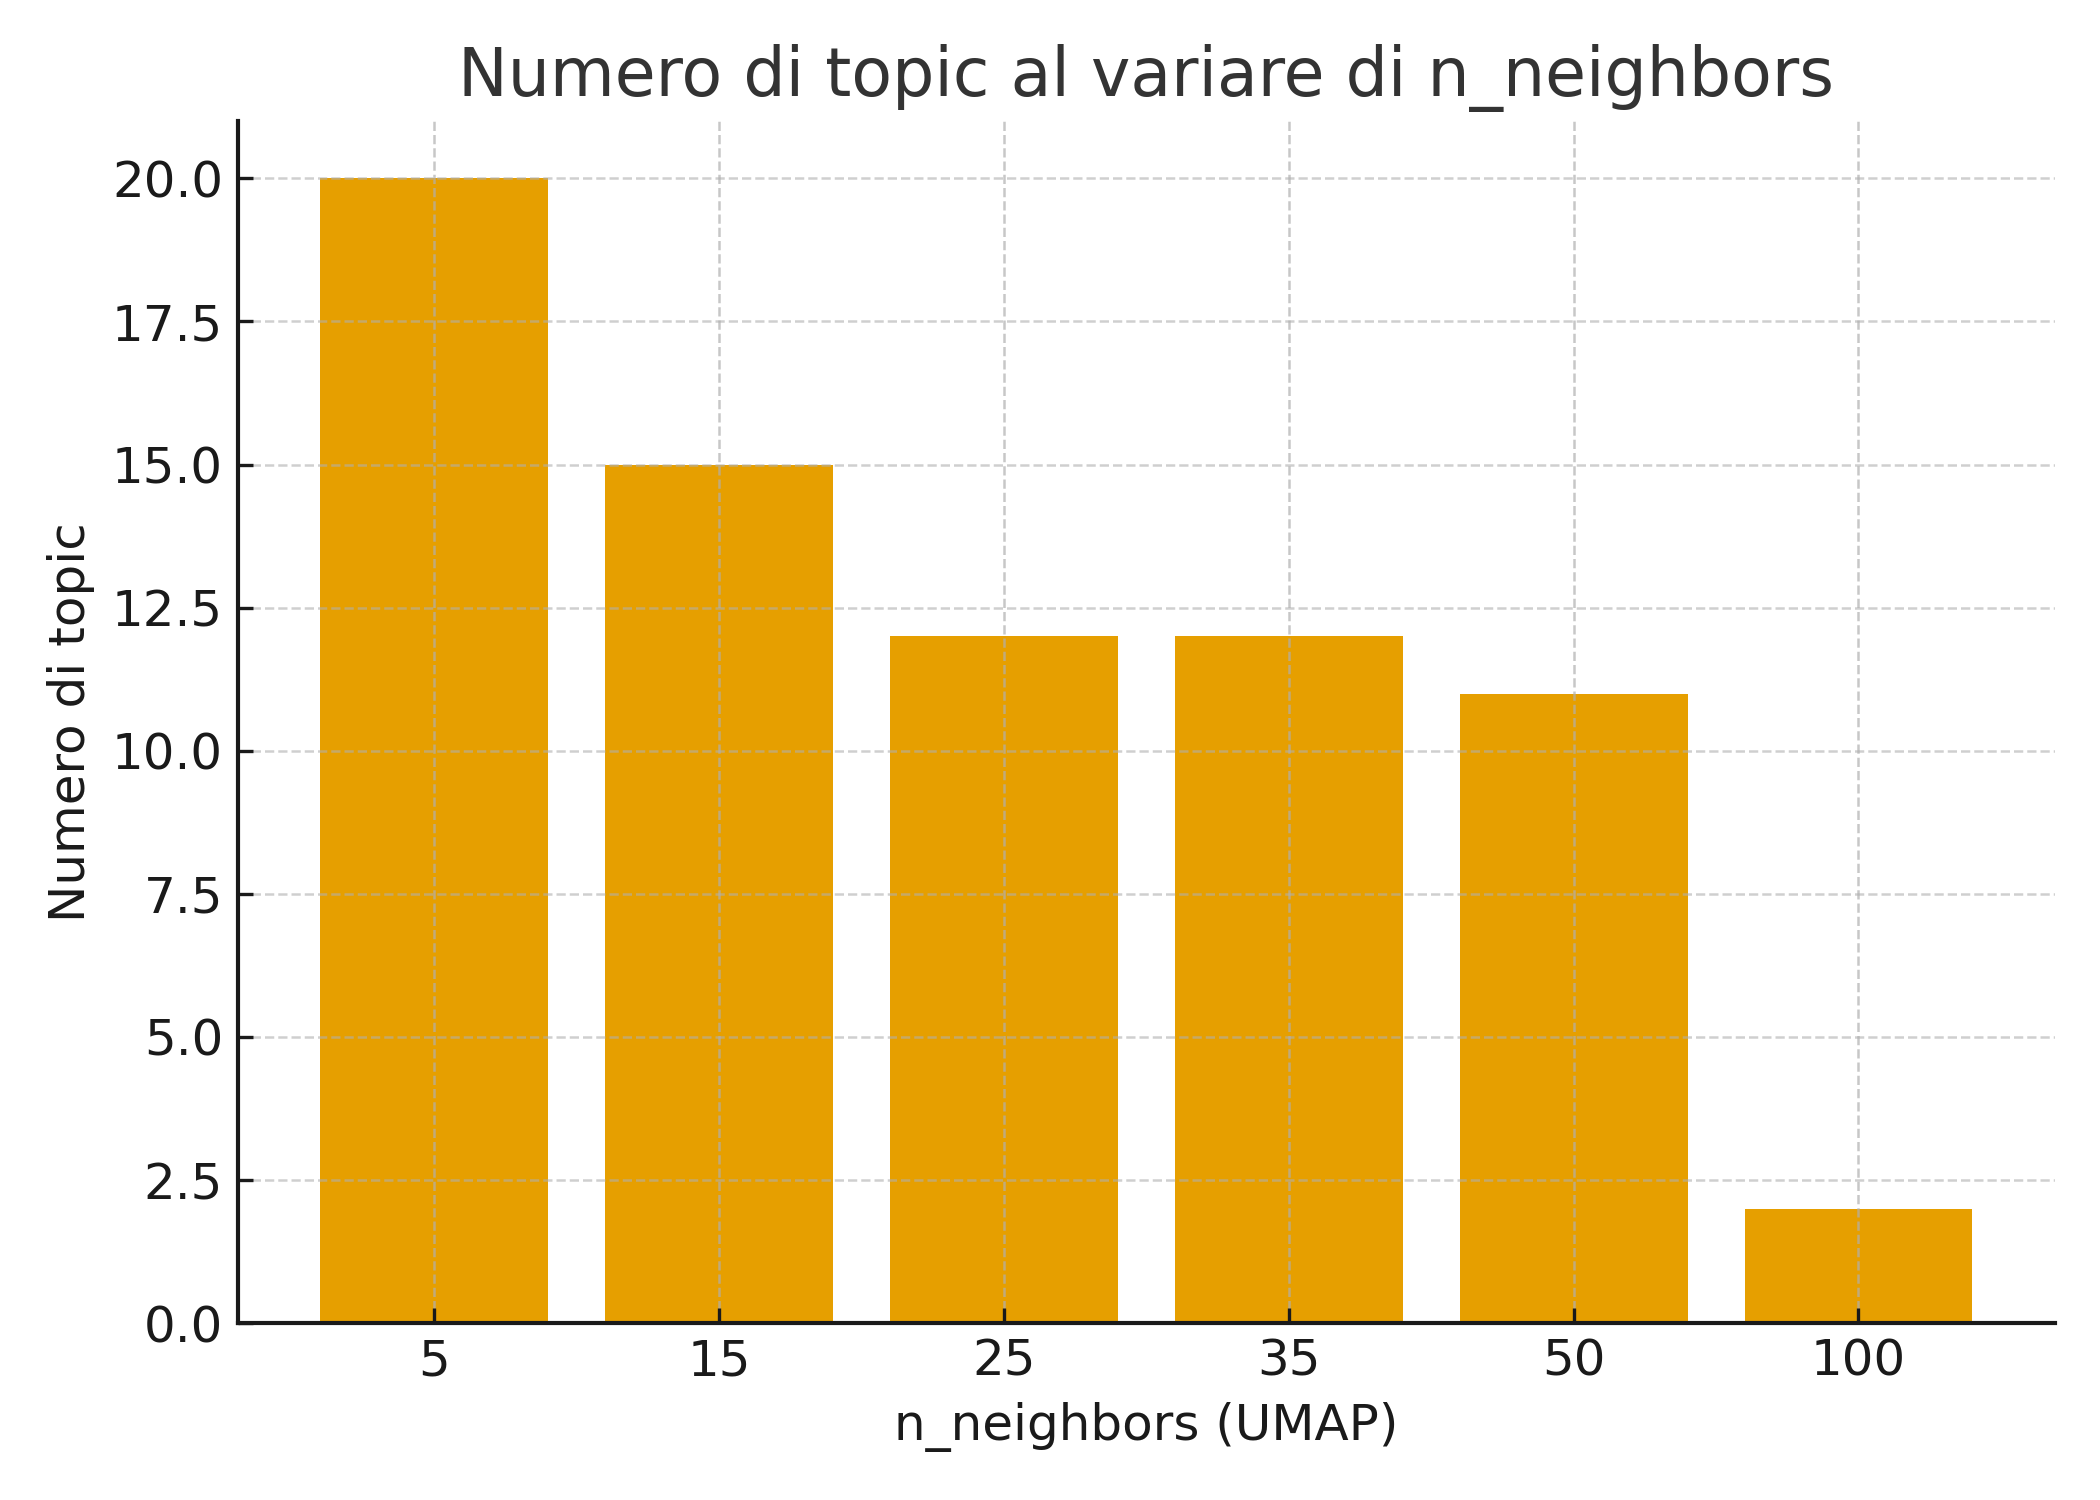
\includegraphics[width=0.6\textwidth]{BERTopic/umap/num_topics_per_neighbors.png}
\caption{Numero di topic generati da HDBSCAN al variare di $n\_neighbors$: la scelta intermedia ($n\_neighbors=50$) massimizza la granularità senza collassare in pochi cluster.}
\label{fig:num-topics-per-neighbors}
\end{figure}
\noindent I plot in Figura~\ref{fig:umap-neighbors-comparison} mostrano la proiezione bidimensionale generata da \texttt{BERTopic.\allowbreak visualize\_documents()} per tre configurazioni distinte. Con \texttt{n\_neighbors} = 15 UMAP costruisce un grafo molto \textbf{frammentato}: le connessioni tra i documenti sono deboli, molti punti rimangono isolati e HDBSCAN li etichetta come \textit{outlier}, generando quindi un topic \texttt{-1} (il topic dove vengono inseriti i documenti di cui si è incerti) estremamente popoloso (2224 documenti). All'estremo opposto (\texttt{n\_neighbors} = 100) il grafo è troppo \textbf{compatto}: le relazioni globali dominano e i topic tendono a fondersi. Con \texttt{n\_neighbors} = 50, invece, i cluster si addensano in regioni coerenti, evidenziando macro-categorie professionali distinte (marketing, cybersecurity, biomedical engineering, \emph{etc.}). L'incrocio tra indicatori numerici e analisi visiva conferma quindi \texttt{n\_neighbors} = 50 come valore finale.

\begin{figure}[H]
\centering
\begin{subfigure}{0.32\textwidth}
    \centering
    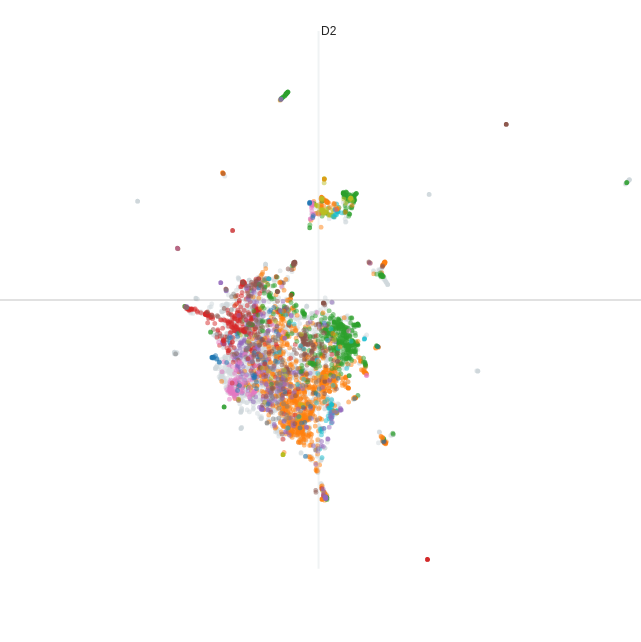
\includegraphics[width=\textwidth]{BERTopic/umap/umap_15.png}
    \caption{$n\_neighbors = 15$}
\end{subfigure}\hfill
\begin{subfigure}{0.32\textwidth}
    \centering
    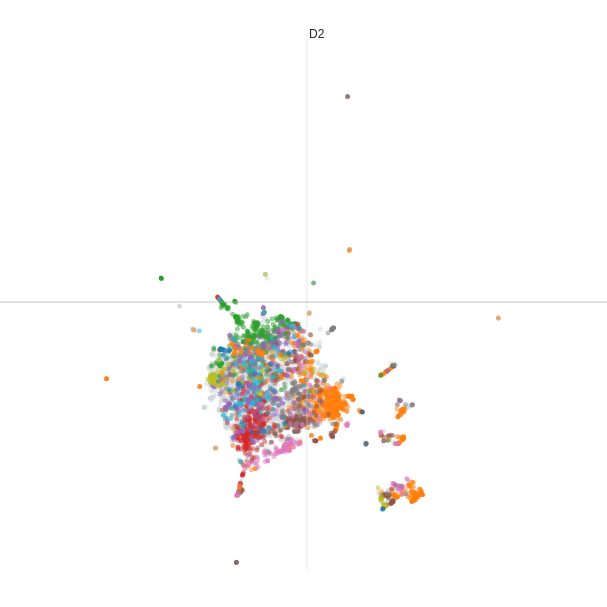
\includegraphics[width=\textwidth]{BERTopic/umap/umap_50.png}
    \caption{$n\_neighbors = 50$}
\end{subfigure}\hfill
\begin{subfigure}{0.32\textwidth}
    \centering
    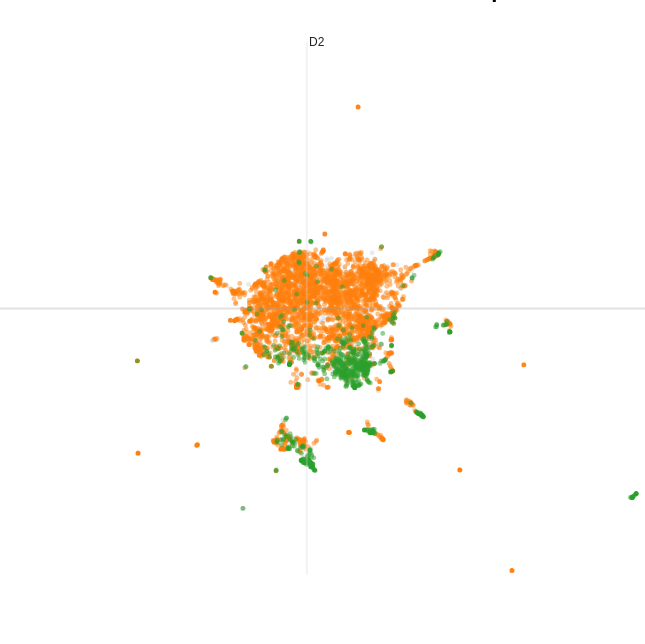
\includegraphics[width=\textwidth]{BERTopic/umap/umap_100.png}
    \caption{$n\_neighbors = 100$}
\end{subfigure}
\caption{Proiezioni generate da \texttt{BERTopic.\allowbreak visualize\_documents()}: i punti (embedding ridotti a 2 dimensioni) sono colorati in base al topic. Confronto tra \texttt{n\_neighbors} pari a 15, 50 e 100.}
\label{fig:umap-neighbors-comparison}
\end{figure}


\paragraph{\texttt{min\_dist}} controlla la densità minima consentita nella proiezione a bassa dimensione. Un valore vicino a zero permette ai punti di collassare in regioni molto dense, mettendo in risalto cluster ben separati; aumentando il parametro, UMAP distribuisce i punti con maggiore uniformità, sacrificando la compattezza dei gruppi a favore di una rappresentazione più omogenea. La Figura~\ref{fig:umap-min-dist} mostra come diverse configurazioni di \texttt{min\_dist} modifichino la distribuzione dei punti: valori estremamente bassi generano isole molto concentrate, mentre impostazioni più elevate distendono l'intero spazio proiettato.
\begin{figure}[H]
\centering

\begin{subfigure}{0.32\textwidth}
    \centering
    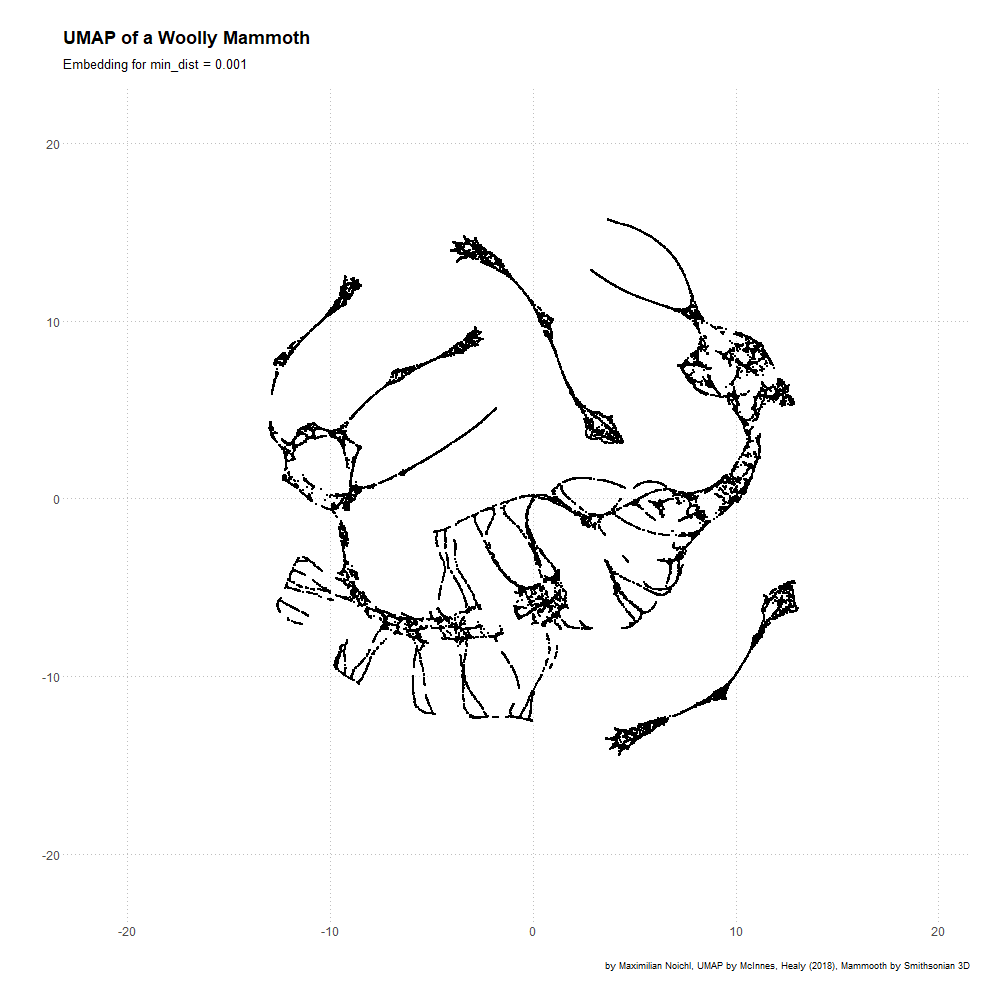
\includegraphics[width=\textwidth]{BERTopic/umap/min_dist_001.png}
    \caption{$min\_dist = 0.01$}
\end{subfigure}\hfill
\begin{subfigure}{0.32\textwidth}
    \centering
    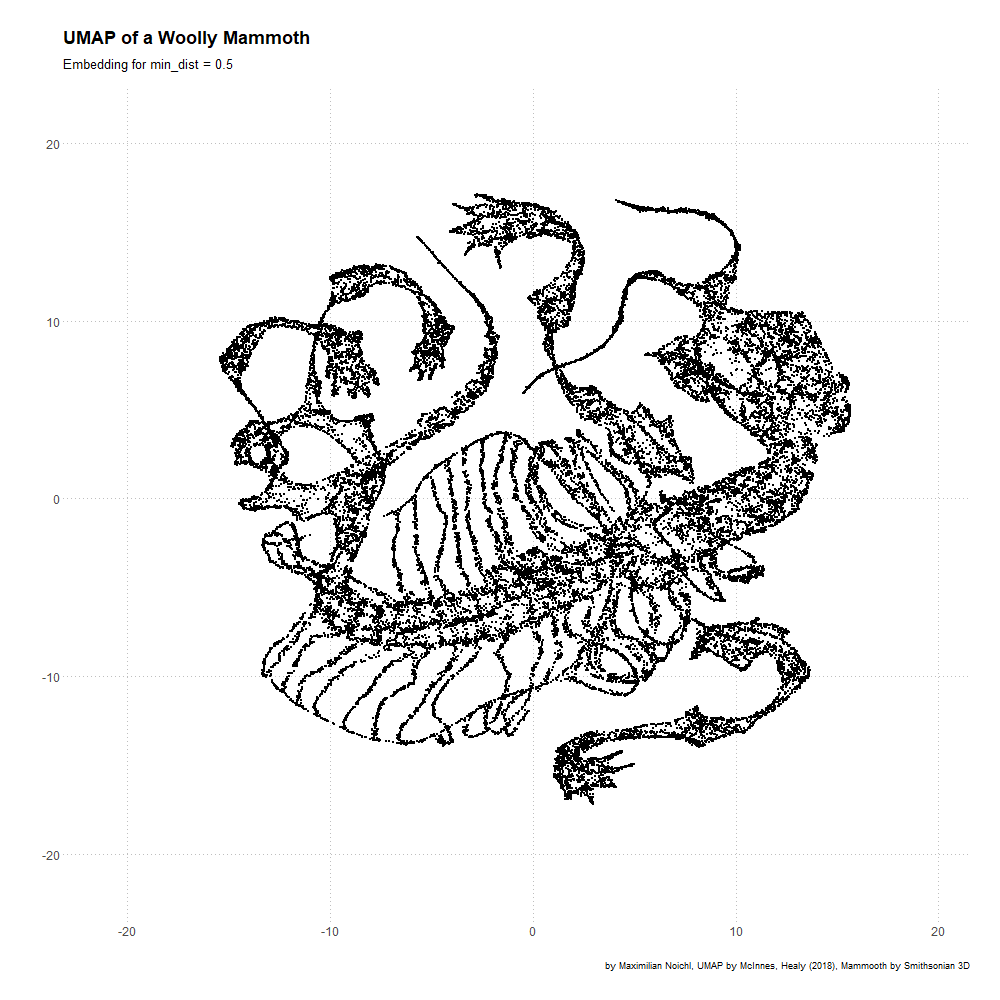
\includegraphics[width=\textwidth]{BERTopic/umap/m_dist_5.png}
    \caption{$min\_dist = 0.5$}
\end{subfigure}\hfill
\begin{subfigure}{0.32\textwidth}
    \centering
    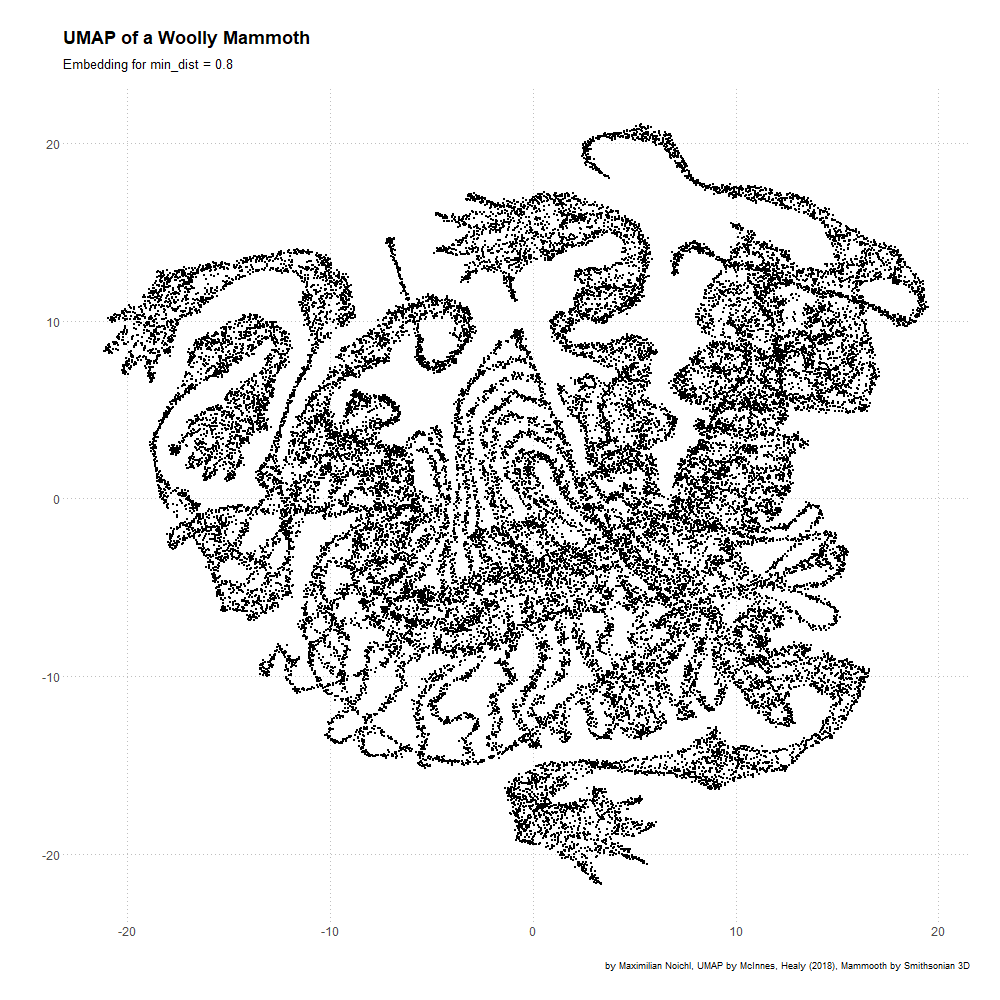
\includegraphics[width=\textwidth]{BERTopic/umap/m_dist_8.png}
    \caption{$min\_dist = 0.8$}
\end{subfigure}
\caption{Effetto di \texttt{min\_dist} sulla proiezione UMAP del modello 3D da 50\,000 punti. Fonti: \href{https://3d.si.edu/object/3d/mammuthus-primigenius-blumbach:341c96cd-f967-4540-8ed1-d3fc56d31f12}{Smithsonian 3D Digitization Program} e \href{https://www.maxnoichl.eu/projects/mammoth/}{Max Noichl}.}
\label{fig:umap-min-dist}
\end{figure}
\noindent Abbiamo fissato \texttt{min\_dist} a $0.0$ poiché l'algoritmo di \emph{clustering} (HDBSCAN) restituisce risultati migliori con cluster densi e ben separati: eventuali regioni vuote verrebbero classificate come outlier e assegnate al topic ``spazzatura'' (\texttt{-1}). Mantenere gli embedding compatti riduce la formazione di tali zone.

\subsection{Clustering}
\noindent Dopo aver ridotto la dimensione dell'input, dobbiamo creare dei \textit{cluster} di embedding simili da cui estrarremo i topic.

\noindent Il modello che consiglia BERTopic\footnote{\url{https://maartengr.github.io/BERTopic/getting_started/clustering/clustering.html}} è \textit{HDBSCAN}, un algoritmo di clustering basato su densità, in modo da identificare cluster a densità variabile senza dover fissare un singolo parametro di soglia (a differenza di \textit{DBSCAN}).

\noindent Il \textit{clustering} viene ottenuto passando per 5 fasi\footnote{\url{https://hdbscan.readthedocs.io/en/latest/how_hdbscan_works.html}}:
\begin{enumerate}
    \item Trasformazione dello spazio basata sulla densità
    \item Minimum spanning tree del grafo pesato delle distanze
    \item Costruzione della gerarchia di aggregazione dei punti
    \item Condensazione della gerarchia in base a \texttt{min\_cluster\_size}
    \item Estrazione dei cluster dall'albero condensato
\end{enumerate}
\subsubsection*{1. Trasformazione dello spazio in funzione della densità}

Il primo passo dell'algoritmo HDBSCAN consiste nel \textit{trasformare lo spazio dei dati} in modo che rifletta non solo la distanza geometrica tra i punti, ma anche la densità locale delle regioni in cui essi si trovano. 
Questo passaggio consente di adattare la nozione di distanza alle caratteristiche strutturali del dataset, migliorando la robustezza rispetto a variazioni di scala e rumore.

Per ogni punto \( x_i \) viene calcolata la \textbf{core distance}, definita come la distanza dal suo \( k\)-esimo vicino più prossimo, dove \( k = \text{min\_samples} \). 
Essa rappresenta una stima della densità locale: valori piccoli indicano aree dense, mentre valori grandi indicano zone più sparse o isolate.

Successivamente, la distanza tra due punti \( a \) e \( b \) viene ridefinita come \textbf{mutual reachability distance}, che tiene conto delle rispettive densità locali:

\[
d_{\text{mreach}}(a,b) = \max \big( \text{core\_dist}(a),\ \text{core\_dist}(b),\ d(a,b) \big)
\]
dove $d(a,b)$ è la distanza originale tra $a$ e $b$. Usando questa distanza, i punti densi rimangono alla loro distanza originale, mentre quelli rarefatti vengono allontanati, ciò rende l'algoritmo \textbf{robusto al rumore}.
Abbiamo però introdotto un parametro \texttt{min\_samples}: al suo crescere aumenta la \texttt{core\_distance} media e con essa i punti considerati rarefatti.
Quindi più è alto \texttt{min\_samples}, più embedding verranno considerati come \textit{rumore}.
Come per \texttt{n\_neighbors}, mostriamo qui dei confronti con diversi valori di \texttt{min\_samples}:

\begin{table}[H]
\centering
\footnotesize
\begin{tabular}{rrrrrrrrr}
\hline
min\_samples & n\_topics & noise \% & mean size & median size & max size & top topic \% & outlier \\
\hline
5  & 12 & 42.28 & 257.67 & 190.0 & 882  & 28.53  & 2265 \\
15 & 61 & 45.88 & 224.98 & 131.0 & 1581 & 11.52 & 11635 \\
30 & 10 & 39.69 & 323.10 & 209.0 & 886  & 27.42  & 2126 \\
60 & 2  & 14.80 & 2282.00 & 2282.0 & 3699 & 81.05  & 793  \\
\hline
\end{tabular}
\caption{Metriche chiave al variare di \texttt{min\_samples}: numero di topic (n\_topics), percentuale di rumore (noise), statistiche di dimensione dei cluster, quota del topic principale e conteggio degli outlier.}
\label{tab:min-samples-summary}
\end{table}
Per valori molto bassi (\texttt{min\_samples} = 5) l'algoritmo tende a frammentare eccessivamente il corpus, generando numerosi micro-cluster spesso composti da pochi paragrafi. 
Sebbene questa impostazione aumenti il livello di dettaglio, i topic risultano meno stabili e semanticamente meno coerenti.

Aumentando il parametro a valori intermedi (\texttt{min\_samples} = 15) si ottiene un equilibrio tra granularità e stabilità. 
I cluster formati risultano sufficientemente omogenei e interpretabili, mantenendo al contempo un numero di topic adeguato per una lettura tematica fine del corpus. 
Questo valore rappresenta il compromesso ottimale tra dettaglio informativo e robustezza del clustering.

Con valori più elevati (\texttt{min\_samples} = 30) l’algoritmo diventa più selettivo: la quantità di rumore aumenta e alcuni cluster tendono a fondersi, riducendo la capacità di distinguere tematiche affini ma distinte. 
Spingendosi ulteriormente verso valori molto alti (\texttt{min\_samples} = 60) si osserva un drastico calo del numero di cluster e un incremento marcato dei punti etichettati come rumore, con il rischio di ottenere pochi macro-temi troppo generici.

\begin{figure}[H]
\centering
\begin{subfigure}{0.24\textwidth}
    \centering
    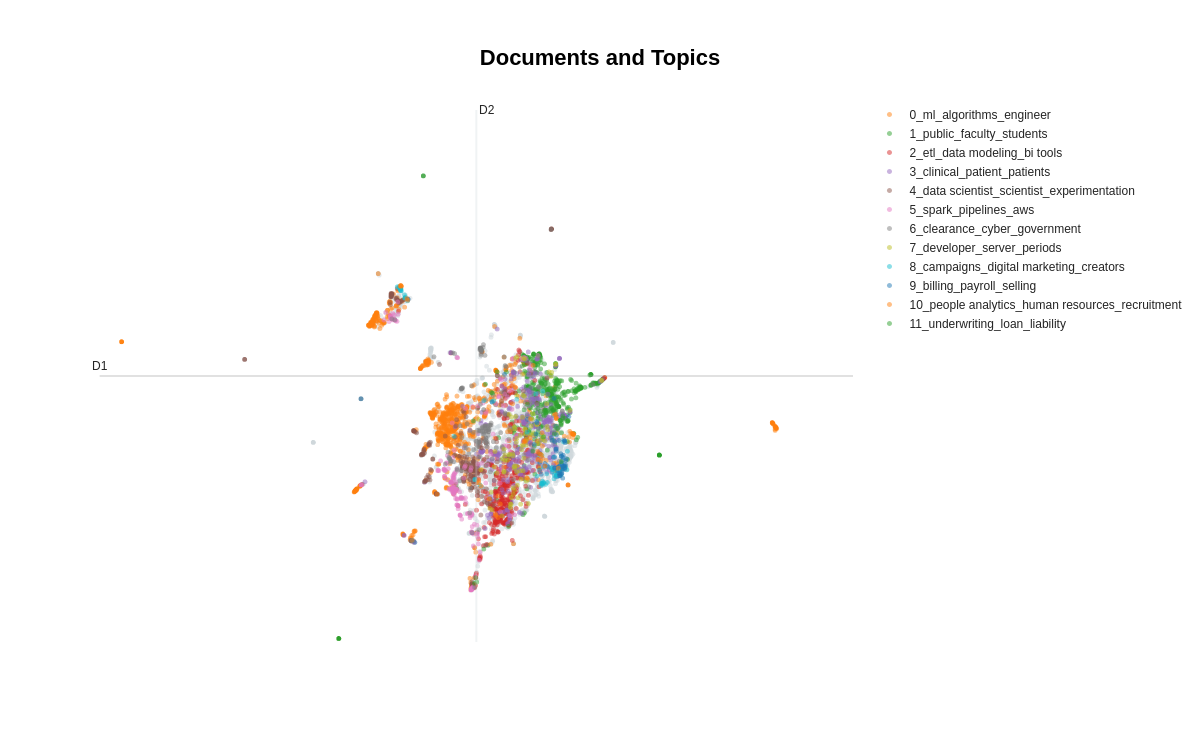
\includegraphics[width=\textwidth]{BERTopic/hdbscan/ms5.png}
    \caption{\texttt{min\_samples} = 5}
\end{subfigure}\hfill
\begin{subfigure}{0.24\textwidth}
    \centering
    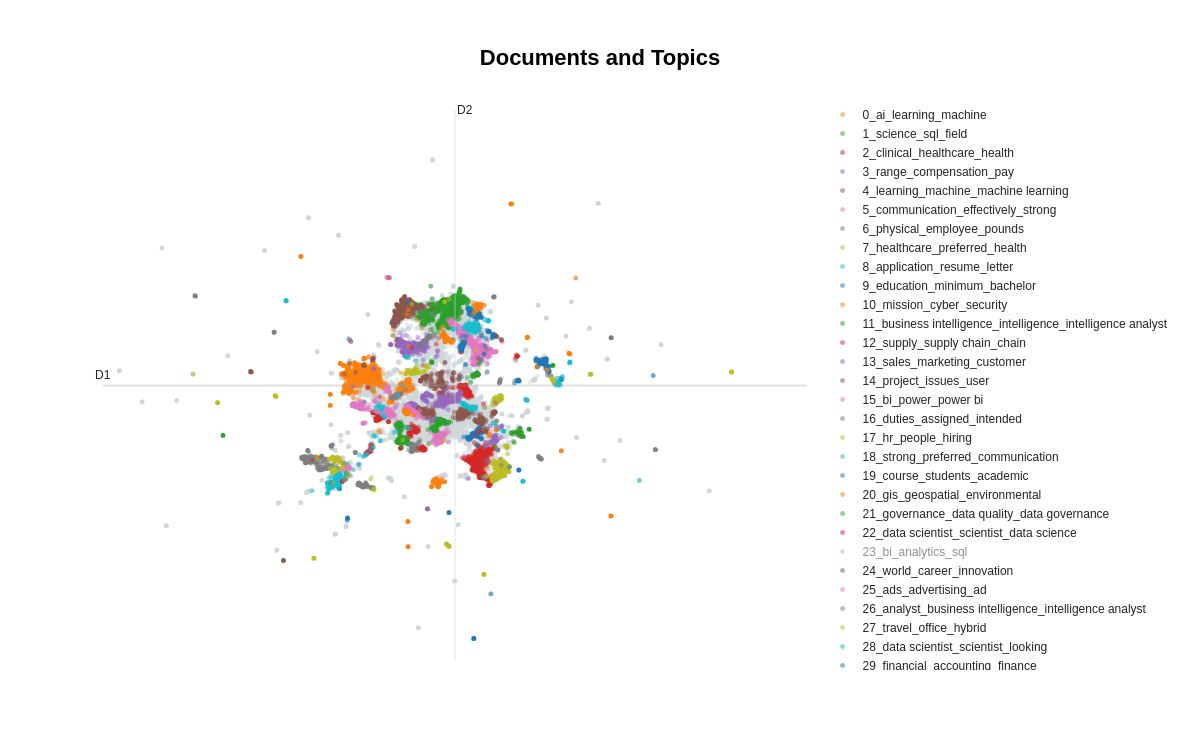
\includegraphics[width=\textwidth]{BERTopic/hdbscan/ms15.png}
    \caption{\texttt{min\_samples} = 15}
\end{subfigure}\hfill
\begin{subfigure}{0.24\textwidth}
    \centering
    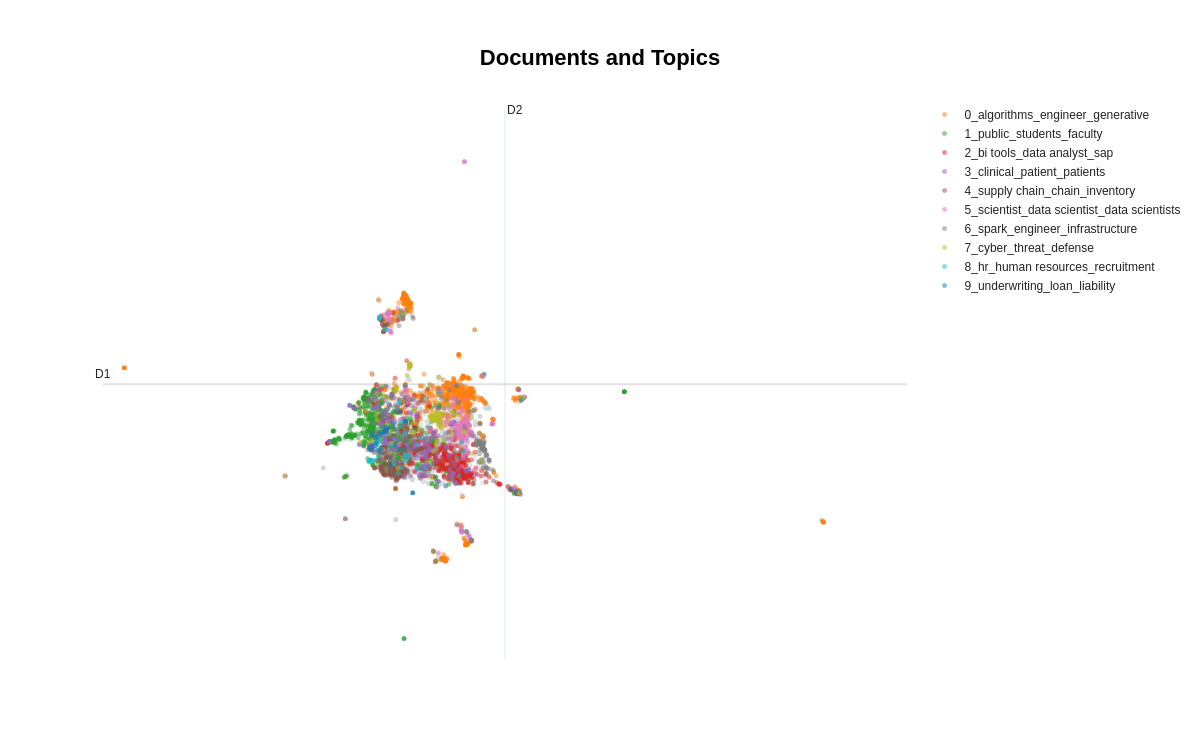
\includegraphics[width=\textwidth]{BERTopic/hdbscan/ms30.png}
    \caption{\texttt{min\_samples} = 30}
\end{subfigure}\hfill
\begin{subfigure}{0.24\textwidth}
    \centering
    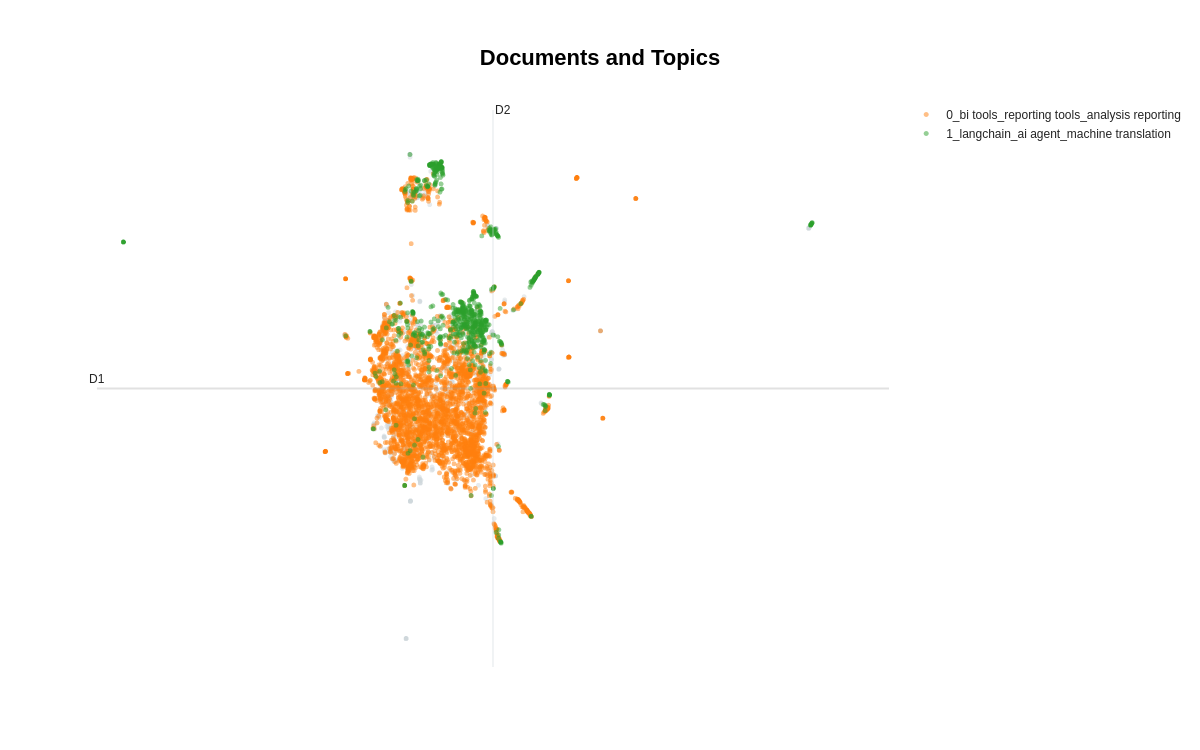
\includegraphics[width=\textwidth]{BERTopic/hdbscan/ms_60.png}
    \caption{\texttt{min\_samples} = 60}
\end{subfigure}
\caption{Effetto di \texttt{min\_samples} sulla distribuzione dei topic: visualizzazioni prodotte da \texttt{BERTopic.visualize\_documents()} in configurazioni crescenti del parametro.}
\label{fig:min-samples-umap}
\end{figure}

Nel complesso, la configurazione con \texttt{min\_samples} = 15 si è dimostrata la più bilanciata: 
garantisce la formazione di cluster stabili, coerenti e sufficientemente dettagliati, risultando quindi la scelta più appropriata per il corpus di annunci di lavoro considerato.

\subsubsection*{2. Costruzione del \textit{Minimum Spanning Tree} (MST)}

Dopo la trasformazione dello spazio in funzione della densità locale, HDBSCAN costruisce un grafo completamente connesso in cui ogni punto rappresenta un nodo e ogni arco tra due punti è pesato in base alla \textit{mutual reachability distance} calcolata nel passo precedente. 
Questo grafo descrive la struttura di connettività del dataset, tenendo conto sia della distanza geometrica sia della densità locale delle regioni considerate.

A partire da tale grafo, viene poi calcolato il \textbf{Minimum Spanning Tree} (MST), ossia l'albero di connessioni che collega tutti i punti minimizzando la somma complessiva dei pesi degli archi. 
Il MST conserva quindi solo le connessioni essenziali per mantenere la connettività globale, eliminando i collegamenti ridondanti e le connessioni tra regioni scarsamente dense.

Questo passaggio ha due obiettivi principali:
\begin{itemize}
    \item \textbf{Semplificare la struttura dei dati}, riducendo la complessità del grafo e mantenendo una rappresentazione compatta della topologia di densità;
    \item \textbf{Preparare la costruzione della gerarchia dei cluster}, poiché nei passi successivi gli archi del MST verranno rimossi in ordine crescente di distanza per individuare i gruppi di punti che restano connessi, ossia i futuri cluster.
\end{itemize}

il Minimum Spanning Tree dunque connette i punti più vicini secondo la loro densità locale e costituisce la base per la costruzione della gerarchia dei cluster nel passo successivo.

\subsubsection*{3. Costruzione della gerarchia dei cluster}

A partire dal \textit{Minimum Spanning Tree} costruito nel passo precedente, HDBSCAN procede alla \textbf{costruzione di una gerarchia di cluster} basata sulle componenti connesse del grafo. 
Questo processo consiste nel rimuovere progressivamente gli archi del MST in ordine crescente di peso, ovvero dalla connessione più ``debole'' (distanza maggiore) a quella più ``forte'' (distanza minore).

Man mano che gli archi vengono rimossi, il grafo si frammenta in un numero crescente di componenti connesse. 
Ogni componente risultante viene interpretata come un potenziale cluster a un determinato livello di densità. 
In questo modo, HDBSCAN genera una \textit{gerarchia di densità} in cui i cluster ``nascono'' e ``muoiono'' al variare della soglia di distanza, descrivendo come la struttura dei dati cambia al modificarsi del livello di densità considerato.

Il risultato di questa fase è un albero gerarchico che rappresenta la relazione di inclusione tra cluster: 
le radici corrispondono ai cluster più generali (densità minore), mentre i rami e le foglie rappresentano i cluster più specifici e densi. 
Questa rappresentazione gerarchica è fondamentale per le fasi successive, poiché consente di identificare in modo naturale i livelli di densità più stabili e significativi all'interno del dataset.

\subsubsection*{4. Condensazione della gerarchia dei cluster}

Una volta costruita la gerarchia completa delle componenti connesse, HDBSCAN applica un processo di \textbf{condensazione} basato sul parametro \texttt{min\_cluster\_size}. 
L'obiettivo è semplificare la struttura gerarchica, eliminando i rami instabili e i cluster di dimensioni troppo ridotte per essere considerati significativi.

Durante questa fase, la gerarchia dei cluster viene attraversata e vengono mantenuti soltanto quei gruppi che rispettano la dimensione minima richiesta. 
I cluster che non raggiungono la soglia stabilita vengono rimossi oppure fusi con componenti più grandi a densità simile, producendo una rappresentazione compatta e più interpretabile della struttura dei dati.

Il risultato di questa operazione è una \textit{condensed tree}, ossia un albero di condensazione in cui ogni nodo rappresenta un cluster potenzialmente stabile e ogni arco riflette una relazione di inclusione o fusione tra cluster. 
Questo passaggio riduce notevolmente la complessità della gerarchia originale, preservando solo le regioni dello spazio che presentano un'evidente coesione interna e scartando i gruppi effimeri o rumorosi.

La condensazione costituisce quindi la base per la successiva selezione dei cluster più stabili, che rappresentano le strutture di densità realmente persistenti all'interno del dataset.
\subsubsection*{5. Estrazione dei cluster stabili dalla struttura condensata}

Dopo aver ottenuto l'albero di condensazione, HDBSCAN seleziona i \textbf{cluster più stabili} in base alla loro persistenza lungo i diversi livelli di densità. 
Ogni cluster nella struttura condensata è caratterizzato da un intervallo di esistenza: esso ``nasce'' quando si separa da un cluster padre e ``muore'' quando, aumentando la soglia di densità, si frammenta o scompare.

Per ciascun cluster, HDBSCAN calcola una misura di \textbf{stabilità} che quantifica la sua persistenza all'interno della gerarchia. 
Tale stabilità corrisponde all'area sotto la curva che descrive l'evoluzione della dimensione del cluster in funzione della densità: 
cluster che permangono per un ampio intervallo di densità sono considerati più stabili e quindi più rappresentativi della struttura intrinseca dei dati.

Durante questa fase, vengono mantenuti soltanto i cluster con una stabilità elevata, mentre i punti appartenenti a regioni meno dense o a cluster transitori vengono etichettati come \textit{rumore} (label~$-1$). 
Questo approccio consente di identificare automaticamente le strutture di densità più consistenti, senza richiedere la specifica del numero di cluster a priori.

\subsection{Tokenizer}
Dettagliare il tokenizer utilizzato, le strategie di pre-processing e qualsiasi personalizzazione per il dominio degli annunci di lavoro.

\subsection{Cosa si può migliorare}
Discutere criticità note, possibili ottimizzazioni della pipeline e idee per estensioni future di BERTopic nel progetto.
